\subsubsection{Speedup Analysis}
\label{subsec:speedup-analysis}
Figire \ref{fig:speed-comparison} shows the runtime ratios.
The left panel shows $T_{\mathrm{ns3sionna}}/T_{\mathrm{sionnart}}$ and a larger value means that \texttt{sionnart} is faster than \texttt{ns3sionna}.
The right panel shows $T_{\mathrm{sionnart}}/T_{\mathrm{pure\ ns3}}$ and a value below one means that \texttt{sionnart} is faster than \texttt{pure\_ns-3} baseline.
The same results are show in Table \ref{tab:speed-comparison}.

\begin{figure}[t]
    \centering
    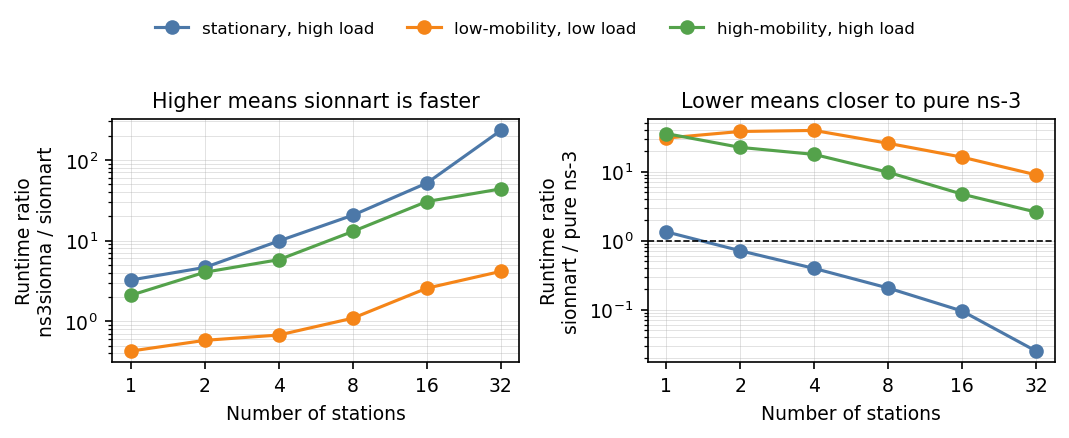
\includegraphics[width=\linewidth]{images/speed_comparison.png}
    \caption{The left graph shows the ratio of \texttt{ns3sionna} runtime to \texttt{sionnart} runtime.
        The right graph is the ratio of \texttt{sionnart} runtime to \texttt{pure\_ns-3} baseline runtime.}
    \label{fig:speed-comparison}
\end{figure}

According to these ratios, embedding Sionna RT using pybind11 helps to improve the performance of simulation.
In two server design, a cache miss must send data from ns-3 to a separate Python process and wait for the reply.
In the embedded design, ns-3, the cache, Sionna RT, all run inside the same process.
This removes much of the communication cost and the remaining cost is the actual ray-tracing, which is still needed when the experiment uses site-specific propagation.

\begin{table}[t]
    \centering
    \caption{Ratios at $N=32$. The first ratio is
    $T_{\mathrm{ns3sionna}}/T_{\mathrm{sionnart}}$; the second is
    $T_{\mathrm{sionnart}}/T_{\mathrm{pure\ ns3}}$.}
    \label{tab:speed-comparison}
    \setlength{\tabcolsep}{5pt}
    \begin{tabular}{lrr}
        \hline
        Scenario                 & Speedup over  & Cost relative \\
                                 & ns3sionna     & to pure ns-3  \\
        \hline
        Stationary, high load    & $232.3\times$ & $0.025\times$ \\
        Low mobility, low load   & $4.15\times$  & $9.00\times$  \\
        High mobility, high load & $43.8\times$  & $2.59\times$  \\
        \hline
    \end{tabular}
\end{table}

However, two server design is also have its own merits.
Having separate server for Sionna RT allows us to run the ray-tracing engine on a different machine, and it also allows us to run multiple ray-tracing engines in parallel.
But for our use case, we only need to run the ray-tracing engine on the same machine as ns-3.
So we choose the embedded design.